\documentclass[tikz,border=10pt]{standalone}

\begin{document}
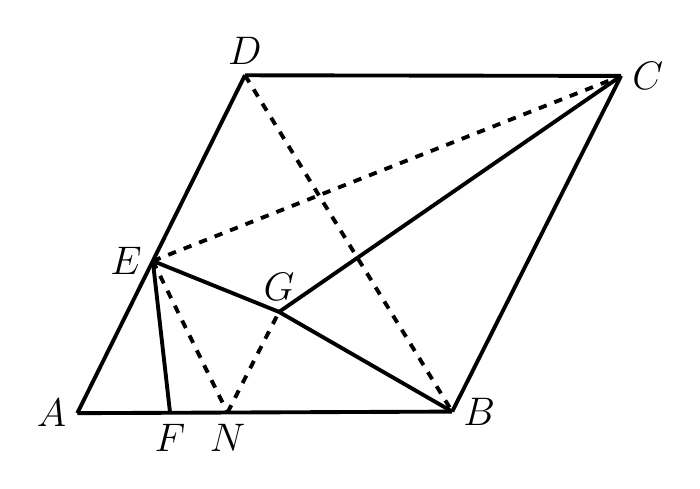
\begin{tikzpicture}[line join=round, line width=1.4pt]
\coordinate (A) at (-3.475,-2.136);
\coordinate (B) at (1.286,-2.116);
\coordinate (C) at (3.431,2.147);
\coordinate (D) at (-1.346,2.155);
\coordinate (F) at (-2.297,-2.131);
\coordinate (G) at (-0.913,-0.850);
\coordinate (N) at (-1.568,-2.129);


\coordinate (E) at (-2.516,-0.203);


\draw (A) -- (B);            
\draw (B) -- (C);            
\draw (C) -- (D);            
\draw (A) -- (E) -- (D);     
\draw (E) -- (G) -- (B);     
\draw (C) -- (G);            
\draw (E) -- (F);            


\draw[dashed] (E) -- (C);
\draw[dashed] (D) -- (B);
\draw[dashed] (N) -- (G);
\draw[dashed] (E) -- (N);


\node[above, font=\fontsize{14.5}{17.4}\selectfont] at (D) {$D$};
\node[right, font=\fontsize{14.5}{17.4}\selectfont] at (C) {$C$};
\node[left, font=\fontsize{14.5}{17.4}\selectfont] at (E) {$E$};
\node[above, font=\fontsize{14.5}{17.4}\selectfont] at (G) {$G$};
\node[left, font=\fontsize{14.5}{17.4}\selectfont] at (A) {$A$};
\node[right, font=\fontsize{14.5}{17.4}\selectfont] at (B) {$B$};
\node[below, font=\fontsize{14.5}{17.4}\selectfont] at (F) {$F$};
\node[below, font=\fontsize{14.5}{17.4}\selectfont] at (N) {$N$};
\end{tikzpicture}
\end{document}